% ===== PIPELINE FIGURE (v3: three stacked panels) — paste where the figure should go =====
% Preamble needs:  \usepackage{tikz} \usepackage{graphicx} \usepackage{adjustbox} \usepackage{float}
%                  \usetikzlibrary{arrows.meta, positioning, calc, decorations.pathreplacing}
% Real numbers come from figstats.tex + data/*.dat (written by make_figure_data.py).
% Without them the figure still compiles, with XX / placeholder curves.
% (tikz libraries are loaded in the preamble)

% ---------------- numbers shown in the figure ----------------
\IfFileExists{figstats.tex}{\input{figstats.tex}}{}
\providecommand{\figNGames}{32}      \providecommand{\figNTeams}{48}
\providecommand{\figYears}{2019--2025}
\providecommand{\figNClips}{5{,}571} \providecommand{\figMeanClip}{XX}
\providecommand{\figCost}{\$0.06}
\providecommand{\figNRaw}{11{,}142}  \providecommand{\figNKept}{10{,}362}
% KDE panels
\providecommand{\figMedClose}{7}  \providecommand{\figXminClose}{2} \providecommand{\figXmaxClose}{14} \providecommand{\figTicksClose}{4,8,12}
\providecommand{\figMedDur}{4}    \providecommand{\figXminDur}{0}   \providecommand{\figXmaxDur}{12}   \providecommand{\figTicksDur}{0,5,10}
\providecommand{\figMedLat}{3}    \providecommand{\figXminLat}{0}   \providecommand{\figXmaxLat}{10}   \providecommand{\figTicksLat}{0,4,8}
% example huddle in panel (c): times in s, spreads in ft
\providecommand{\exXmax}{10}  \providecommand{\exYmax}{12}
\providecommand{\exXticks}{0,5,10} \providecommand{\exYticks}{0,5,10}
\providecommand{\exThr}{5.8}                       % "tight" cutoff
\providecommand{\exTin}{3.6}  \providecommand{\exTout}{7.3}   % enters / leaves tight zone
\providecommand{\exTmin}{5.3} \providecommand{\exSmin}{3.7}   % tightest moment
\providecommand{\exSzero}{10.8}                      % spread when the point ends

% ---------------- image helpers ----------------
\providecommand{\vbimg}[2]{%
  \IfFileExists{images/#2}%
    {\includegraphics[width=#1]{images/#2}}%
    {\tikz\node[draw=black!30, fill=black!5, minimum width=#1,
       minimum height=0.6*#1, font=\tiny\ttfamily, text=black!50]{\edef\vbtmp{#2}\detokenize\expandafter{\vbtmp}};}%
}
\ifdefined\vbbox\else\newsavebox{\vbbox}\fi
\providecommand{\vbimgcr}[4]{% height, crop fraction per side, file, corner radius
  \IfFileExists{images/#3}%
    {\sbox{\vbbox}{\adjustbox{trim={#2\width} 0pt {#2\width} 0pt, clip, height=#1}%
       {\includegraphics{images/#3}}}%
     \tikz{\clip[rounded corners=#4] (0,0) rectangle (\wd\vbbox,{\ht\vbbox+\dp\vbbox});
           \node[anchor=south west, inner sep=0pt] at (0,0) {\usebox{\vbbox}};}}%
    {\tikz\node[draw=black!30, fill=black!5, rounded corners=#4, minimum width=1.42*#1,
       minimum height=#1, font=\tiny\ttfamily, text=black!50]{\detokenize{#3}};}%
}

% ---------------- square images for the four moments ----------------
% \vbcover: scale until the image fills the square, then trim equal amounts from both
%           edges (keeps the centre, no stretching).
% \vbfit:   show the whole image at its true shape, with white padding in the square.
% Pick one in \vbsqimg below.
\ifdefined\vbsqbox\else\newsavebox{\vbsqbox}\fi
\ifdefined\vbtx\else\newlength{\vbtx}\newlength{\vbty}\fi
\providecommand{\vbmissing}[1]{{\tiny\ttfamily\color{black!50}\edef\vbtmp{#1}\detokenize\expandafter{\vbtmp}}}
\providecommand{\vbcover}[2]{%
  \IfFileExists{images/#2}{%
    \sbox{\vbsqbox}{\includegraphics[height=#1]{images/#2}}%
    \ifdim\wd\vbsqbox<#1\relax\sbox{\vbsqbox}{\includegraphics[width=#1]{images/#2}}\fi
    \setlength{\vbtx}{\dimexpr(\wd\vbsqbox-#1)/2\relax}%
    \setlength{\vbty}{\dimexpr(\ht\vbsqbox+\dp\vbsqbox-#1)/2\relax}%
    \clipbox{{\vbtx} {\vbty} {\vbtx} {\vbty}}{\usebox{\vbsqbox}}%
  }{\vbmissing{#2}}%
}
\providecommand{\vbfit}[2]{%
  \IfFileExists{images/#2}%
    {\includegraphics[width=#1, height=#1, keepaspectratio]{images/#2}}%
    {\vbmissing{#2}}%
}
\providecommand{\vbsqimg}{\vbcover}   % <- change to \vbfit for whole image + padding

\definecolor{accent}{RGB}{150,120,210}
\definecolor{teamA}{RGB}{226,96,64}
\definecolor{curvecol}{RGB}{214,48,49}   % match the circle colour in your BEV images
\definecolor{teamB}{RGB}{70,110,210}

% Placed exactly here ([H]). Put \clearpage BEFORE the section header, not here.
\begin{figure}[H]
\centering
\adjustbox{max width=\textwidth, max totalheight=0.5\textheight}{%
\begin{tikzpicture}[
    >={Stealth[length=2.6mm, width=2mm]},
    flow/.style    ={->, line width=0.9pt, black!80},
    dflow/.style   ={flow, dashed},
    ptitle/.style  ={font=\Large\bfseries, anchor=north west},
    stage/.style   ={rectangle, rounded corners=10pt, fill=black!6, draw=none},
    clipfile/.style={rectangle, rounded corners=4pt, fill=accent!15, draw=accent,
                     line width=0.7pt, minimum width=3.4cm, minimum height=0.8cm,
                     font=\ttfamily\Large\bfseries},
    lab/.style     ={font=\Large, text=black!85, align=center},
    stat/.style    ={font=\large, text=black!55, align=center},
    divider/.style ={black!25, line width=1pt},
    handoff/.style ={->, accent!85!black, line width=1.6pt, rounded corners=10pt},
    hchip/.style   ={rectangle, rounded corners=5pt, fill=white, draw=accent!85!black,
                     line width=1pt, inner sep=5pt, font=\large,
                     text=accent!60!black, align=center},
]
\def\W{30}   % canvas width (cm)
%
% =====================================================================
% (a) FINDING HUDDLES
% =====================================================================
\node[ptitle] (ta) at (0,0) {(a) Finding the huddles {\mdseries\color{black!50} (in each of the \figNGames\ games)}};
%
% pile of game videos
\foreach \dx/\dy/\f/\nm in {-0.35/0.35/berry_emory.png/pileA, 0/0/laverne_southwestern.png/pileB, 0.35/-0.35/hope_calvin.png/pileC}
  \node[fill=white, draw=black!35, inner sep=1.5pt] (\nm) at ({3.6+\dx},{-3.2+\dy}) {\vbimg{4.8cm}{\f}};
\node[lab, font=\Large\bfseries, anchor=north] (games) at ($(pileC.south -| 3.6,0)+(0,-0.3)$) {\figNGames\ games};
\node[stat, below=0pt of games] {D-III women's volleyball\\\figYears\ $\cdot$ \figNTeams\ teams};
%
% segmentation
\node[stage, minimum width=11.0cm, minimum height=4.6cm] (seg) at (14.85,-3.5) {};
\node[lab, font=\Large\bfseries] at ($(seg.north)+(0,-0.5)$) {Huddle clipping};
\node (gem) at ($(seg.center)+(-2.8,0.15)$) {\vbimg{1.5cm}{gemini.png}};
\node (hum) at ($(seg.center)+( 2.8,0.15)$) {\vbimg{1.5cm}{user.png}};
\node[font=\LARGE\bfseries] at ($(gem)!0.5!(hum)$) {+};
\node[below=3pt of gem, font=\ttfamily\normalsize, align=center] {gemini-3.1\\-pro-preview};
\node[below=3pt of hum, font=\large, text=black!75, align=center] {person checks\\\& fixes};
\node[stat, below=4pt of seg] {\figCost\ per huddle};
\draw[flow] ($(pileC.east |- seg.west)+(0.3,0)$) -- ($(seg.west)+(-0.25,0)$);
%
% clips
\def\cx{25.6}
\node[stat, align=center] at (\cx,-0.95) {one game $\to$ up to 5 sets,\\$\sim$45 huddle clips per set};
\node[clipfile] (c1) at (\cx,-2.0) {H1\_S1.mp4};
\node[clipfile] (c2) at (\cx,-3.1) {H2\_S1.mp4};
\foreach \dy in {-0.2,0,0.2} \fill[black!70] (\cx,{-4.05+\dy}) circle (1.6pt);
\node[clipfile] (c4) at (\cx,-5.0) {H23\_S5.mp4};
\coordinate (fan) at ($(seg.east)+(0.3,0)$);
\foreach \c in {c1,c2,c4} \draw[flow] (fan) -- ($(\c.west)+(-0.15,0)$);
\draw[dflow] (fan) -- (\cx-1.9,-4.05);
%
%
%
% =====================================================================
% (b) LOCATING PLAYERS
% =====================================================================
\node[ptitle] (tb) at (0,-7.7) {(b) Locating the players {\mdseries\color{black!50} (in each of the \figNClips\ clips)}};
\def\by{-12.25}   % vertical centre of panel (b) content
%
% FIX 1: photos spread apart so "homography" fits between them
\node[inner sep=0pt] (courtimg) at (3.6,\by) {\vbimgcr{5.0cm}{0.10}{white_court.png}{12pt}};
\node[lab, below=5pt of courtimg] {\textbf{1.} find the court lines};
\node[inner sep=0pt] (playerimg) at (13.9,\by) {\vbimgcr{5.0cm}{0.10}{player_track.png}{12pt}};
\node[lab, below=5pt of playerimg] {\textbf{2.} find every player};
\draw[flow] ($(courtimg.east)+(0.2,0)$) -- ($(playerimg.west)+(-0.2,0)$)
     node[midway, above, font=\large, text=black!55] {homography};
%
% top-down court map (18 m x 9 m)
\def\cs{0.5556}
\coordinate (mapSW) at (19.6,{\by-2.5});
\begin{scope}[shift={(mapSW)}, x=\cs cm, y=\cs cm]
  \fill[black!4] (0,0) rectangle (18,9);
  \draw[black!45, line width=0.7pt] (0,0) rectangle (18,9);
  \draw[black!40, line width=0.5pt] (6,0) -- (6,9) (12,0) -- (12,9);
  \draw[black!80, line width=1.8pt] (9,-0.5) -- (9,9.5);
  % one frame, both teams, court coordinates in metres
  \foreach \px/\py in {8.15/0.41, 8.11/2.41, 6.54/8.09, 5.7/1.56, 4.47/6.22, 2.18/4.18}
    \fill[teamA] (\px,\py) circle (3pt);
  \draw[teamA, line width=1.1pt] (6.25,4.02) circle (4.08);
  \foreach \px/\py in {12.26/2.25, 9.67/2.43, 10.47/3.74, 9.91/5.9, 13.03/6.67}
    \fill[teamB] (\px,\py) circle (3pt);
  \draw[teamB, line width=1.1pt] (11.35,4.55) circle (2.71);
  \coordinate (mapNE) at (18,9);
\end{scope}
\node[inner sep=0pt, minimum width={18*\cs cm}, minimum height={9*\cs cm}, anchor=south west] (map) at (mapSW) {};
\node[lab, below=5pt of map] (maplbl) {\textbf{3.} map every player onto the court, frame by frame (ft)};
\draw[flow] ($(playerimg.east)+(0.2,0)$) -- ($(map.west)+(-0.2,0)$);
%
%
%
% hand-off (a) -> (b): every clip runs through the same steps
\def\laneA{-8.95}
\draw[handoff] ($(c4.south)+(0,-0.15)$) -- (\cx,\laneA) -- (courtimg.north |- 0,\laneA)
     -- ($(courtimg.north)+(0,0.15)$);
\node[hchip] at ($(courtimg.north |- 0,\laneA)!0.5!(\cx,\laneA)$) {all \figNClips\ clips from the \figNGames\ games};
%
% =====================================================================
% (c) MEASURING EACH HUDDLE
% =====================================================================
\node[ptitle] (tc) at (0,-16.4) {(c) Measuring each huddle {\mdseries\color{black!50} (one example, then all \figNKept)}};
%
\begin{scope}[yshift=-1.9cm]
%
% ---- filmstrip: four moments, game video on top, bird's-eye view below ----
\def\sq{2.2cm}          % side of each square frame
\def\sqin{2.2cm}                   % size of the image inside the square
\tikzset{sqframe/.style={rectangle, inner sep=0pt, minimum width=\sq, minimum height=\sq,
          draw=black!30, line width=0.5pt, rounded corners=3pt, fill=white}}
\def\fytop{-17.68}      % top of the video images
% images: images/moment1_video.png, images/moment1_bev.png, ... moment4
% FIX 2: frames 3.7 cm apart (was 3.5) and labels at \large (was \Large)
\foreach \nm/\fs/\x/\word/\t in {fA/moment1/2.6/point ends/0, fB/moment2/6.3/huddle forms/\exTin,
                             fC/moment3/10.0/tightest/\exTmin, fD/moment4/13.7/breaks up/\exTout} {
  \node[sqframe, anchor=north] (\nm vid) at (\x,\fytop)
       {\vbsqimg{\sqin}{\fs_video.png}};
  \node[sqframe, anchor=north] (\nm bev) at ($(\nm vid.south)+(0,-0.15)$)
       {\vbsqimg{\sqin}{\fs_bev.png}};
  \coordinate (\nm) at (\nm bev.south);
  \node[lab, anchor=south, font=\large] at ($(\nm vid.north)+(0,0.1)$)
       {\textbf{\word}\\[-1pt]{\large $t=\t$\,s}};
}
\node[font=\large, text=black!60, rotate=90, anchor=south] at ($(fAvid.west)+(-0.1,0)$) {video};
\node[font=\large, text=black!60, rotate=90, anchor=south] at ($(fAbev.west)+(-0.1,0)$) {bird's-eye};
%
% ---- spread over time for that huddle ----
\pgfmathsetmacro{\xu}{11.6/\exXmax}   % cm per second
\pgfmathsetmacro{\yu}{3.6/\exYmax}    % cm per foot
\begin{scope}[shift={(2.2,-26.63)}, x=\xu cm, y=\yu cm]
  % duration: time spent below the cutoff
  \fill[accent!16] (\exTin,0) rectangle (\exTout,\exYmax);
  % axes, ticks, labels
  \draw[black!60, line width=0.7pt, -{Stealth[length=1.8mm]}] (0,0) -- ({1.04*\exXmax},0);
  \draw[black!60, line width=0.7pt, -{Stealth[length=1.8mm]}] (0,0) -- (0,{1.08*\exYmax});
  \foreach \tk in \exXticks
    \draw[black!60, line width=0.6pt] (\tk,0) -- ++(0,-4pt)
         node[below, font=\large, text=black!70] {\tk};
  \foreach \tk in \exYticks
    \draw[black!60, line width=0.6pt] (0,\tk) -- ++(-4pt,0)
         node[left, font=\large, text=black!70] {\tk};
  \node[font=\Large, text=black!80] at ({0.5*\exXmax},0) [yshift=-1.05cm] {time since the point ended (s)};
  \node[font=\Large, text=black!80, rotate=90] at (0,{0.5*\exYmax}) [yshift=1.05cm] {enclosing circle (ft)};
  % duration
  \draw[accent!80!black, line width=1.1pt, {Stealth[length=2mm]}-{Stealth[length=2mm]}]
       (\exTin,{0.93*\exYmax}) -- (\exTout,{0.93*\exYmax})
       node[midway, above, font=\Large\bfseries, text=accent!70!black] {duration};
  % the curve (real huddle from data/example_huddle.dat if present)
  \IfFileExists{data/example_huddle.dat}%
    {\draw[curvecol, line width=1.6pt, line join=round] plot file {data/example_huddle.dat};}%
    {\draw[curvecol, line width=1.6pt] plot[smooth, tension=0.6] coordinates
       {(0,10.8) (1,10.1) (2,8.6) (3,6.8) (3.8,5.4) (4.6,4.3) (5.3,3.7) (6.1,4.0)
        (6.9,5.0) (7.6,6.5) (8.5,8.4) (9.5,9.9)};}
  % latency: from the point ending to the tightest moment
  \draw[accent!80!black, line width=1.4pt] (0,{0.08*\exYmax}) -- (\exTmin,{0.08*\exYmax});
  \draw[accent!80!black, line width=1.4pt] (\exTmin,{0.04*\exYmax}) -- (\exTmin,{0.12*\exYmax});
  \draw[accent, dashed, line width=0.7pt] (\exTmin,\exSmin) -- (\exTmin,{0.08*\exYmax});
  \node[above, font=\Large\bfseries, text=accent!70!black] at ({0.5*\exTmin},{0.08*\exYmax}) {latency};
  % closeness: the smallest spread
  \node[circle, fill=accent, inner sep=3pt] at (\exTmin,\exSmin) {};
  \node[anchor=west, font=\Large\bfseries, text=accent!70!black] at ({\exTmin+0.15},{0.27*\exYmax}) {closeness};
  % where each frame sits on the curve
  \coordinate (pA) at (0,\exSzero);
  \coordinate (pB) at (\exTin,\exThr);
  \coordinate (pC) at (\exTmin,\exSmin);
  \coordinate (pD) at (\exTout,\exThr);
\end{scope}
\foreach \f/\p in {fA/pA, fB/pB, fC/pC, fD/pD} {
  \draw[accent, densely dotted, line width=1.1pt] ($(\f)+(0,-0.1)$) -- (\p);
  \fill[accent] (\p) circle (2.2pt);
}
%
%
% ---- distributions over all huddles (your own KDE images), stacked ----
\def\kw{4.6cm} \def\kh{3.45cm}   % box each KDE image is fitted into (aspect ratio kept)
% FIX 4: shorter heading so it clears "breaks up" and "Play-by-play data"
\node[lab, font=\Large\bfseries] at (19.4,-16.8) {Across all \figNKept\ huddles};
\foreach \nm/\y in {closeness/-18.98, duration/-22.55, latency/-26.12}
  \node[inner sep=0pt, minimum width=\kw, minimum height=\kh] (kde\nm) at (19.4,\y)
       {\IfFileExists{images/kde_\nm.png}%
          {\includegraphics[width=\kw, height=\kh, keepaspectratio]{images/kde_\nm.png}}%
          {\tikz\node[draw=black!30, fill=black!5, minimum width=\kw, minimum height=\kh,
             font=\tiny\ttfamily, text=black!50]{kde\_\nm.png};}};
% FIX 3: arrow starts clear of the (moved) last frame
\draw[flow] (15.1,-22.55) -- ($(kdeduration.west)+(-0.25,0)$)
     node[midway, above, font=\large, text=black!65] {repeat};
%
% ---- the three features feed one data set ----
\draw[decorate, decoration={brace, amplitude=9pt}, line width=0.9pt, black!70]
     ($(kdecloseness.north east)+(0.3,0)$) -- ($(kdelatency.south east)+(0.3,0)$);
% FIX 5: wider box so "latency" isn't hyphenated
\node[stage, text width=6.3cm, align=left, inner sep=8pt] (out) at (27.1,-23.35)
     {{\Large\bfseries Final data set}\\[3pt]
      {\large \figNKept\ rows}\\[-1pt]
      {\normalsize\color{black!55}one per team per huddle}\\[7pt]
      {\normalsize\color{black!55}huddle features}\\[-1pt]
      {\large closeness $\cdot$ duration $\cdot$ latency}\\[5pt]
      {\normalsize\color{black!55}from play-by-play}\\[-1pt]
      {\large score $\cdot$ who won the point}};
%
% ---- play-by-play data feeds in from above ----
\node[lab, font=\Large\bfseries] (pbplbl) at (27.1,-16.8) {Play-by-play data};
\def\pw{5.0cm} \def\ph{3.0cm}   % box the play-by-play image is fitted into (aspect ratio kept)
\node[inner sep=0pt, anchor=north, minimum width=\pw, minimum height=\ph] (pbp) at ($(pbplbl.south)+(0,-0.15)$)
     {\IfFileExists{images/pbp.png}%
        {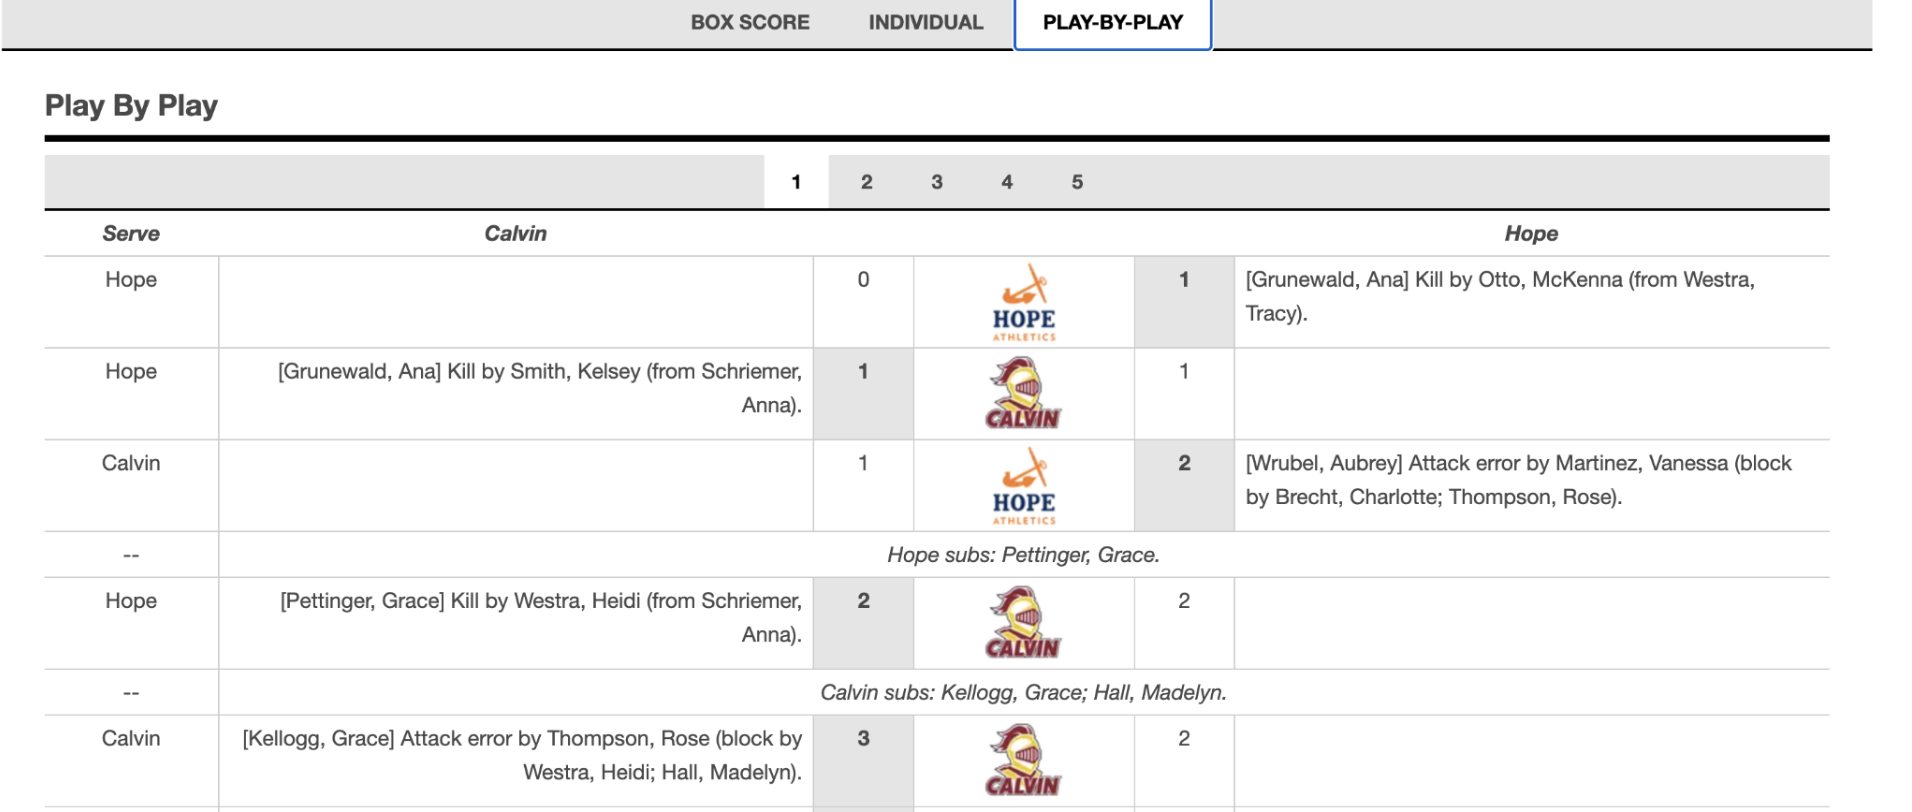
\includegraphics[width=\pw, height=\ph, keepaspectratio]{images/pbp.png}}%
        {\tikz\node[draw=black!30, fill=black!5, minimum width=\pw, minimum height=\ph,
           font=\tiny\ttfamily, text=black!50]{pbp.png};}};
\draw[flow] ($(pbp.south)+(0,-0.12)$) -- ($(out.north)+(0,0.12)$);
\draw[flow] ($(kdeduration.east)+(0.95,0)$) -- ($(out.west |- kdeduration.east)+(-0.2,0)$);
\end{scope}
% hand-off (b) -> (c): the frame-by-frame data feed the per-huddle measurements
\def\laneC{-17.7}
\draw[handoff] ($(maplbl.south)+(0,-0.1)$) -- (maplbl.south |- 0,\laneC) -- (8.15,\laneC) -- (8.15,-18.15);
\node[hchip] at ($(8.15,\laneC)!0.5!(maplbl.south |- 0,\laneC)$) {\figNRaw\ $\to$ \figNKept\ team-huddles after filtering};
%
\end{tikzpicture}%
}
\caption{\textbf{(a)} We collected 32 NCAA Division III women’s volleyball games (2019–2025) from YouTube. We prompted an MLLM (gemini-3.1-pro-preview) to identify start and stop times for every post-point huddle, and a human reviewed each answer using a labeling tool. Games had three to five sets, each averaging 45 huddles, except the fifth, which averaged 25. \textbf{(b)} We fed each huddle clip through a two-step video segmentation model (SAM 3): the first step identified the court to build homography for camera distortion correction, and the second detected and tracked on-court players at 30 fps, giving each player’s position in every frame. \textbf{(c)} After removing tracking errors and non-huddle moments, we track the diameter of the smallest circle enclosing a team’s players (red circle, bird’s-eye view) through the break, giving one curve per huddle. We then derive closeness (smallest distance), latency (time to come together), and duration (time staying together). Kernel density plots show each feature’s distribution across all huddles.}
%
\label{fig:pipeline}
\end{figure}
% ===== END PIPELINE FIGURE =====